% !TEX root = ../Rulebook.tex
\label{sec:Competition}

\section{Teams and Roles}
\label{sec: teams and roles}

The TC and OC will jointly determine the number of teams permitted to participate in a competition well in advance. The rules shall enable a competition with up to at least 24 teams lasting not more than four full days. The number of people to register per team is not restricted by default, but may be limited due to local arrangements. Teams that plan to bring more than four members are advised to contact the OC beforehand.

During registration, each team has to designate one member as teamleader. A change of the teamleader must be communicated to the OC. 
The teamleader is the only person who can officially communicate with the referees during the competition, e.g. aborting a run, to call a restart, etc. 
The teamleader may ask the OC to accept additional teammembers for these tasks.

Each team must also nominate one person which acts as a referee during all tests.
The job of each referee is to ensure that the arena state before each performance is the same as the initial run setup.
They also rate the robot performances during a run. 
This ensures that the interests of every team are respected equally.
It also involves the refs in discussions with other teams and the league officials,
which helps getting to know each other.
Each referee gets a referee sheet from the OC which is used to evaluate the performance. An additional referee is the head referee which measures the time and organizes the referees. If less than 4 referees without the head referee are available (so less than 4 teams participate), TC members can also be referees to fill this up to 4. 4 referees are beneficial, because there is at least one on each side of the arena. A referee briefing is held before a competition by the TC and OC. The goal is to discuss questions and to sensitize the referees for their task. Only briefed refs are allowed to judge the future runs. Teams are asked to send at least two members to the briefing, if possible.

Teams are asked (and wished) to comment their robots performance during their run.
This makes the competition more entertaining while also sharing knowledge about robots, 
the challenges of a task and smart solutions.
The commentator may be any teammember and is optional during competitions.

\section{Meetings and Language of Communication}

Both the TC and the OC may organize several special meetings during a competition, 
such as referee meetings, teamleader meetings, etc.
The meetings are held in english and will be planned and announced locally.
They are used to clarify rules, assign timeslots, request test participation or for any other exchange of information between teams and commitee members.
It is the responsibility of each team to inform themselves about the organization and scheduling of such meetings.
Each team is expected to send at least one representative to such meetings. If the meeting refers to specific roles, such as 'referee' or 'team leader', the person designated by the team to fill this role is expected to participate.


\section{Code of Conduct and Disqualification}
Teams and team members are expected to maintain a friendly and cooperative atmosphere throughout a competition and contribute to a vivid work environment and to scientific exchange before, during and after a competition.
\par
The TC may disqualify individual team members or a whole teams during a competition for severe reasons, such as repeated breach of rules.


\section{Competition Procedure}

The competition is held in the form of so called tests.
A test requires a robot to perform various abilities, including navigation, manipulation, task planning and autonomous decision making.
Different kinds of tests each have their focus a current research field, e.g. picking moving objects or efficient task execution.

All tests require a robot to autonomously navigate through the arena defined in \ref{sec:ArenaDesign} without causing a collision. Each team can enter the arena before actual competitions to create a map of the environment and test their robot. The OC will organize time slots for each team respecting the amount of teams and available slots. Usually there will be some setup days that can be used only for training.

\section{Time Schedule}

The actual competition currently includes a total of 7 tests.
These are spread across available competition days with time buffers in between each other.
An example for the schedule can be found here: \url{https://atwork.robocup.org/rc2021/}.
As on site events have tighter schedules and additionally require teams to prepare everything for an unknown environment, there will usually only be two setup and four competition days, maybe even less.
Teams should prepare for something like fig. \ref{fig:example_schedule}. 

\begin{figure}[h!]
\centering
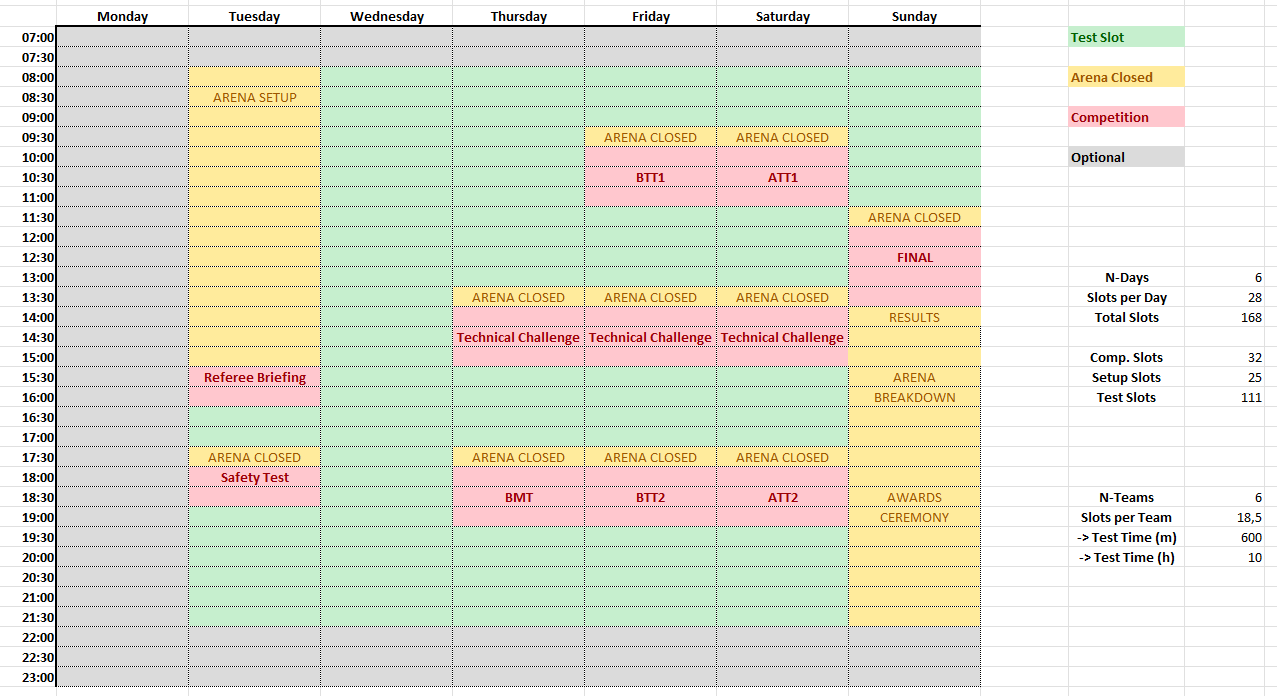
\includegraphics[width= 0.9\textwidth ]{./images/competition/Competition_Schedule_2023.PNG}
\caption{Example of a time schedule for a \RCAW competition.}
\label{fig:example_schedule}
\end{figure}


\section{Practice Slots}

The teams will be given an opportunity to practice with their robots either in the competition arenas or in special test arenas, if available. The frequency and lengths of practice periods will be decided by the OC on site. The OC will also decide about if and how many teams may use an arena simultaneously and can decide on a practice schedule for teams wishing to use the arenas. Arenas may be modified between practice time and competition runs.


\section{Qualification for a Test}
\label{sec:qulaification for a test}

Depending on the amount of participating teams and available timeslots, 
the competition \textbf{may be} seperated into different stages.
Starting with the rather easy tests including all teams, only high performing teams might be allowed to participate in later (more difficult) tests.

The OC must create an onsite schedule during the setup days and announce it before the first competition day. 
The schedule should include all teams in all tests if possible,
but might introduce special stages in the following order:
\begin{enumerate}
\item Stage One: limit the maximum amount of teams in the final test, only the X best teams may participate
\item Stage Two: limit the maximum amount of teams in the Advanced Transportation and later tests, only the X best teams may participate
\end{enumerate}

Teamleaders of qualified teams are required to announce 1 hour before the respective time slot wether their team likes to participate in a test or not. 
This enables the OC to plan the schedule and create scoring sheets.

\section{Parc ferm\'e}

All participating teams must bring their performing robot to the parc ferm\'e 15 minutes before a test and leave them there during the whole timeslot of the test, except when they must perform.
Rules similar to motorsports apply: The robot must not be worked on or changed in any kind unless
serious damage must be repaired. This intends to encourage teams to watch other performances while still give teams the chance to remain in the competition. It is allowed to attach a charger to the robot.

The location of the parc ferm\'e will be towards the spectators for entertainment.
The robots may (are wished to) be turned on and ready to perform, enabling teams to set robot arm positions and illumination for the visitors. 

If the power management of a robot does not enable it to be turned on during the runs of other teams,
the specific team may power-on and boot their robot once the run of the previous team has ended.
They may not change or modify their robot in any way during this time (hardware and software).

\section{Test Procedure}

15 minutes before a competition slot, the arena is set up for the upcoming test.
Therefore, the position of each static arena element is checked and objects are placed on active 
Service Areas.
The TC will decide where dynamic arena elements are placed. See table \ref{fig:test_specifications_instance} for the different responsibilities of placing arena elements, Objects (Pose), Decoys, Containers etc.

A competition slot consists of multiple performance slots (one for each team), 
including a preparation phase, the run phase and the end phase.

\textbf{Preparation Phase}

During the prep phase, teams are allowed to move their robot from the parc ferm\'e to the defined start pose in the arena either by hand or by carefully driving manually. They should prepare their robot for their run and can therefore remote access the robot and/or make minor changes.
It is explicitly forbidden to hardcode solutions for specific requirements of a test during this phase (e.g. drawing position of obstacles in the map). Also, if the robot passes and detects obstacles during this phase, they must be erased from the memory (e.g. clear costmap) unless they can be detected from the START location. The TC might disqualify teams that try to gain unfair advantages from the current or even the following tests.

\clearpage

\textbf{Run Phase}

The run phase begins once the preparation time is up or when the teamleader announces that the team is ready. 
The task is then sent to the robot and from there on, the robot must act fully autonomously. 
It is forbidden to interact or control the robot in any human kind (keyboard/mouse actions, gestures, voice). 
The only interaction allowed is the unplugging of a LAN cable connecting the robot and the controlling pc
when relying on wired communication due to onsite WiFi jams.

During the run phase, the robot must not leave, nor may any person enter the arena.
Teammembers of the performing team are allowed to enter the arena to prevent damage in case of an error (e.g. remove a dropped object from the robots path), but receive a penalty for each interaction.
If a robot behaves uncontrolled and poses a potential threat to the environment,
any person may approach the robot and press the emergency stop.
However, it is requested and strongly advised that only the developers touch their robot.


The run phase regularly ends when:
\begin{itemize}
\item The robot has reached the FINISH location of the arena
\item The run time is up
\item The teamleader says 'stop'
\end{itemize}

The run phase ends early when:
\begin{itemize}
\item The robot has caused a second major collision
\item The emergency stop button had to be pressed before a restart call
\item A team was identified to be cheating 
\end{itemize}

The end of a run phase must be announced by the OC by saying 'end'.
Once this happened, the team may touch and control their robot to bring it to a full stop.

\textbf{End Phase}

In the resulting end phase the team is expected to move their robot back to parc ferm\'e.
Referees gather and discuss their performance rating afterwards.
Once they agree on the performing team's result, 
the teamleader is required to accept this score. 
Teams are allowed to make their case if they do not agree with the refs decision,
but cannot force changes and are expected to be understanding.
Special cases will be decided by the TC if the rulebook leaves room for interpretation.

Once the score has been accepted by a team,
the arena must be set up for the next run if necessary.
The prep time of the next team begins once the arena state is declared as ready by all refs.

\clearpage

\textbf{Performance Slot Example}

\begin{figure} [h!]
	\begin{center}
		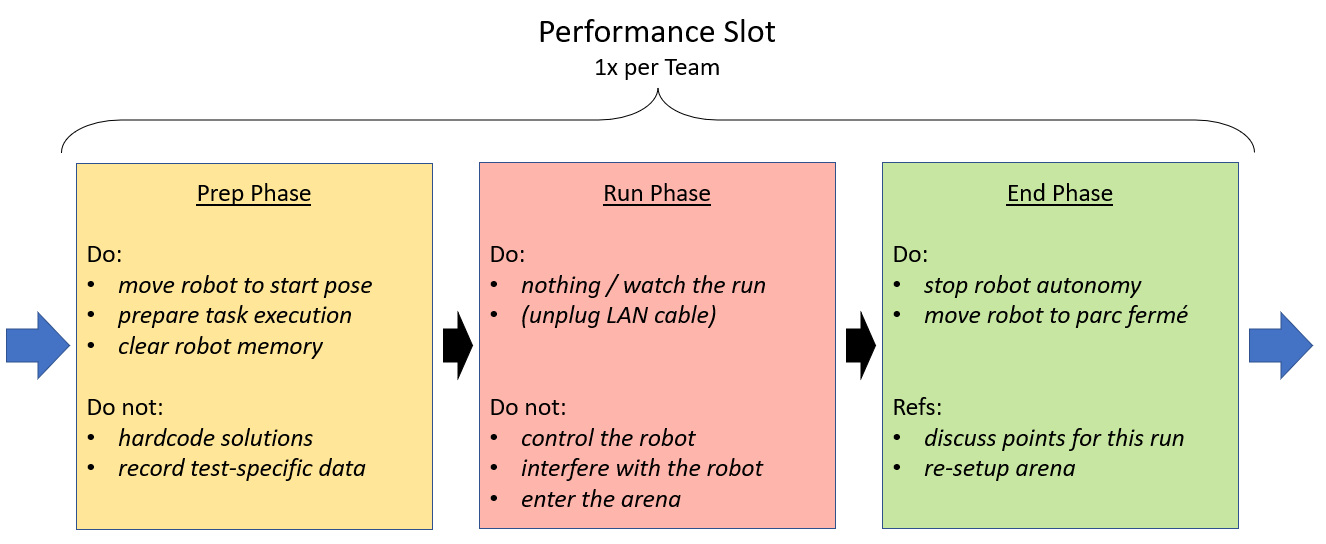
\includegraphics[width= 0.9\linewidth]{./images/competition/performance_slot}
	\end{center}
	\caption{Performance Slot Example: each team gets one per test, following the random team order}
	\label{fig:performance slot example}
\end{figure}



\section{Restarting a Run}
\label{sec:restartingarun}

During a run, the teamleader can restart the test execution once.
Therefore he/she must say 'restart', which stops the current run phase. The robot must be stopped using the emergency switches, which then allows the refs to reset the arena state.
The remaining run time will be noted and used after the restart. Once the refs have finished resetting the arena, the performing team is brought back to their prep phase, which allows them to move the robot back to the start area and prepare it for the restarted run.
A so called tactical call of a restart (e.g. to prevent a major collision) is allowed, because this rewards the teams knowledge about the robot.
Note: When the first major collision occurs, the team can decide whether they stop the run or they restart the run (see section \ref{sec:Collisions}).


\section{Skipping Tests}

If a team decides to not participate in a test during the official time slot, 
they may repeat that test type once in one of the following competition slots.
Their performance slot for the later test type is then replaced by one that suits the previously skipped test type, 
and they then can perform that test type instead of the originally scheduled one.

This should enable struggling teams to do the more simpler tests later in the competition,
but should only be used by teams if it is really necessary in order to keep the structure of the overall competition. 
It is not allowed to repeat a test that has been replaced with this option.

Please note that this option might not be available at all if the schedule is too tight otherwise.

\section{Atwork Commander (AC)}
\label{sec:atwork-commander}

All specific test configurations are being generated using the atwork-commander.

\begin{center}
	\url{https://github.com/robocup-at-work/atwork-commander}
\end{center}

The purpose of the atwork-commander is to create randomized test configurations for any given arena configuration.
It thereby essentially functions as a master control, creating and sending current tasks to robots.
It may also keep time during the prep, run and end phase.
Robots must connect to the atwork-commander using one of the following interfaces:

\paragraph{Object Scoped}
The commander generates transportation tasks for each individual object that must be transported.
This includes the object class and the initial and target service area.
The exact pose of the object is not specified and the order of all transportation tasks is random.

\paragraph{Arena Scoped}
The commander transmits the initial and the target state of the arena.
Service areas each contain the respective objects according to the individual test configuration,
meaning robots must figure out the transportation tasks by themselves.

Robots should remain connected to the AC during their whole test run.
It may be required (optional) to send feedback to the AC (heartbeat, completed tasks).
Please access the github for detailed interface desciptions.

\subsection{On Site}

During a robocup, one unique test configuration is created and being used for each individual test.
All teams must perform this (the same) test configuration in their assigned performance slot.
For training purposes, other configurations may be created and sent to a robot during a test slot of the team.

Depending on the organization and possibilities on site, the TC must either provide all teams with atleast one "public" PC with a running AC to allow them to test their connection setup or decide before the first competition day if only bagfiles are being used.

In this case, robots do not have to connect to the atwork commander during a run, but may rather process the contents of the rosbag and start the task execution.
The run phase of a team then starts once the robot operator announces his starting action (executing a 'rosbag play NAME' command). 



